%****************************************************************%
% FILE: stazioni_osservative_fisse.tex                           %
%****************************************************************%
\documentclass[./main.tex]{subfiles}

\begin{document}
Le stazioni osservative fisse richieste dall'applicazione riguardano le piattaforme poste sul mare. In particolare si dividono in stazioni meteorologiche fisse e radar. Le stazioni sono tutte private, quindi con i dati non completamente disponibili. Mentre i radar hanno dati pubblici accessibili, salvo malfunzionamenti del server fornitore.

% STAZIONI METEROLOGICHE FISSE
\paragraph{Stazioni meteorologiche fisse.}

L'ambiente marino necessita di essere osservato e tutelato. In Italia esistono vari sistemi di osservazione indipendenti che si occupano della raccolta dei dati. In particolare la \textit{Rete Italiana di siti fissi per l’osservazione del mare} (\textbf{IFON}) è composta da diverse piattaforme fisse in grado di trasmettere i dati acquisiti quasi in tempo reale. Esse garantiscono l'osservazione degli ambienti costieri, di mare aperto e profondi, per alcune variabili inserite nelle \textbf{EOV} -- \textit{Essential Ocean Variables}\footcite[5]{rete-ifon}.\par


% rete ifon
%\paragraph{Rete IFON.} 
La rete \textbf{IFON} (\textit{Italian Fixed-point Observatory Network}), composta da 17 infrastrutture costiere e di mare aperto, costituisce un sistema distribuito di monitoraggio a livello nazionale. In \autoref{fig:rete_ifon} è possibile osservare la mappa contenente i siti per l'osservazione del mare appartenenti alla rete.\par

L'applicazione richiede la visualizzazione dei dati provenienti da alcuni impianti della rete, situati nel quadrante nord del mar Adriatico:

\begin{enumerate}
    \item Piattaforma Oceanografica Acqua Alta.
    \item Meda PALOMA.
    \item Meda S1-GB.
    \item Boa meteo oceanografica E1.\par
\end{enumerate}


\begin{figure}[!ht]
\noindent\begin{minipage}{0.5\textwidth}
\vspace{1cm}
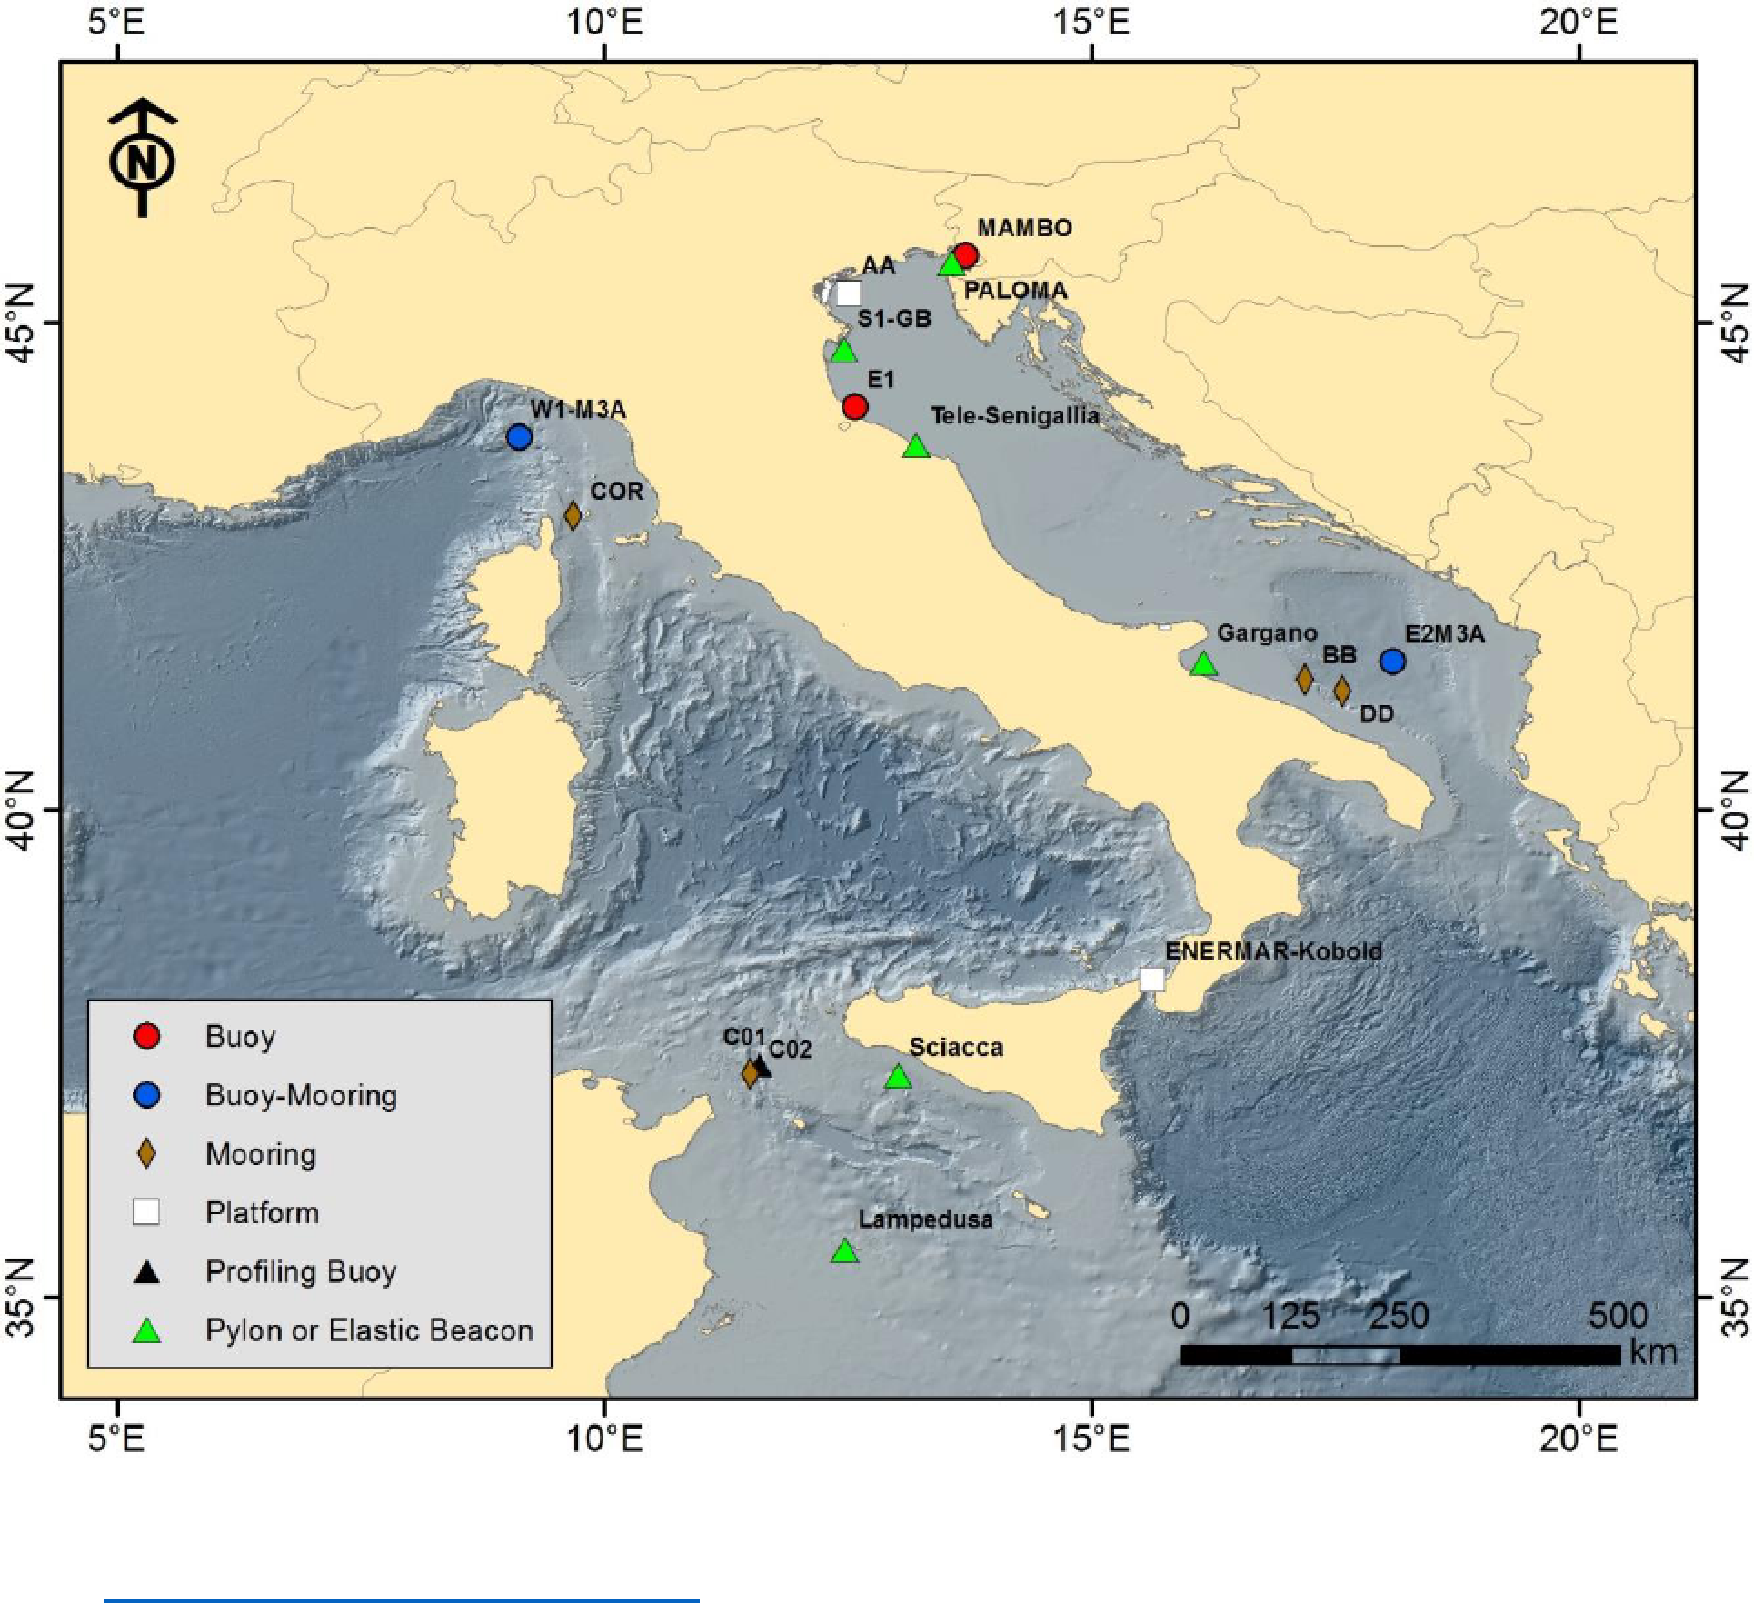
\includegraphics[width=\textwidth]{images/ifon_rete.pdf}
\captionsetup{font=small, hypcap=false}
\captionof{figure}{Mappa rete IFON\footcite[Fonte: ][7]{rete-ifon}.}
\label{fig:rete_ifon}
\end{minipage}
\hspace{0.05\textwidth}
\begin{minipage}{0.4\textwidth}
\begin{small}
Mappa dei siti della rete scientifica italiana di siti fissi per l’osservazione del mare. I tipi di struttura sono indicati nella legenda (Boe, piattaforme, mede, mooring, sistemi profilanti).
\end{small}
\end{minipage}
\vspace{0.25cm}
\end{figure}

Queste strutture verranno brevemente descritte qui di seguito.\par

% piattaforma acqua alta
\begin{figure}[!ht]
\noindent\begin{minipage}{0.5\textwidth}
\vspace{1cm}
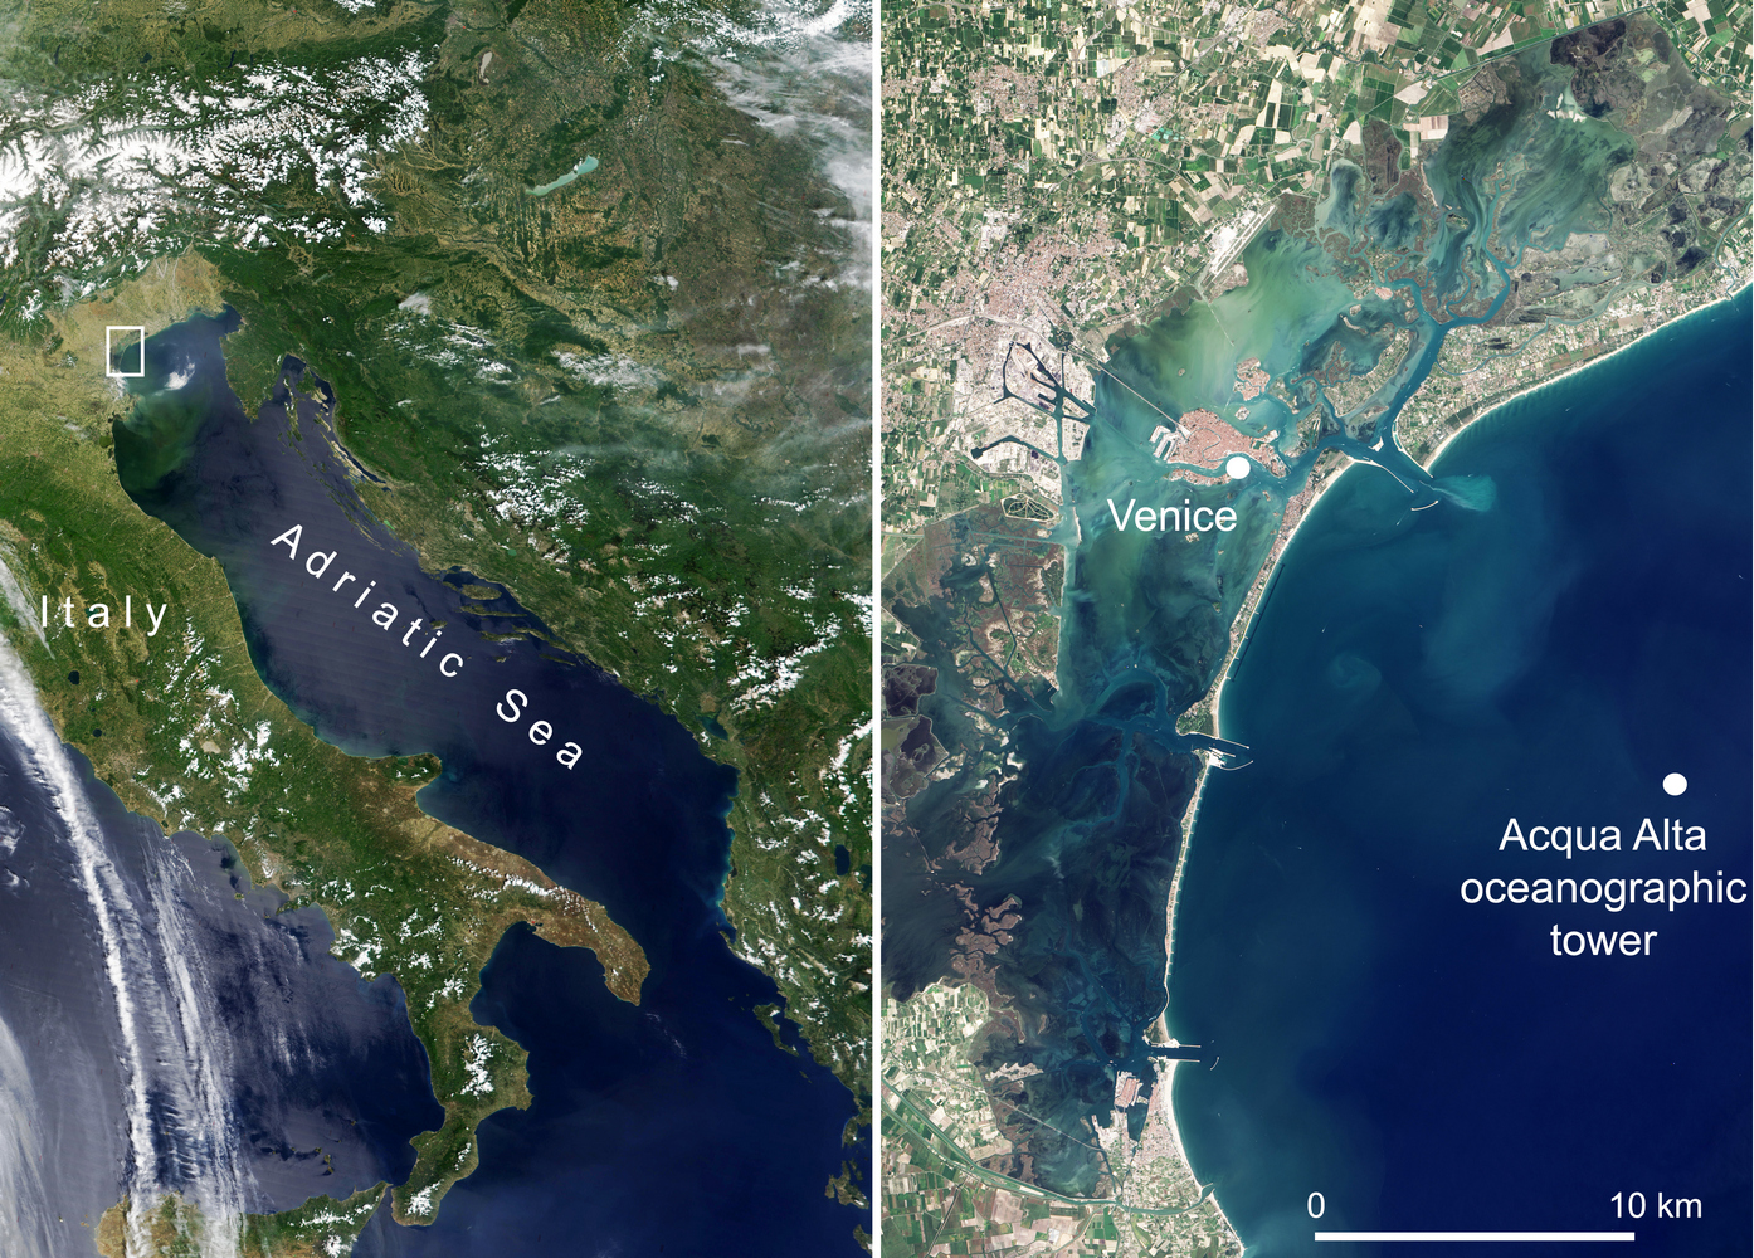
\includegraphics[width=\textwidth]{images/ifon_mappa_aaot.pdf}
\captionsetup{font=small, hypcap=false}
\captionof{figure}{Sito Piattaforma Oceanografica Acqua Alta\footcite[Fonte: ][\url{https://www.ismar.cnr.it/wp-content/uploads/2023/07/mappa-PTF.pdf}]{website-ismar-cnr}.}
\label{fig:ifon_mappa_aaot}
\end{minipage}
\hspace{0.05\textwidth}
\begin{minipage}{0.4\textwidth}
\vspace{1cm}
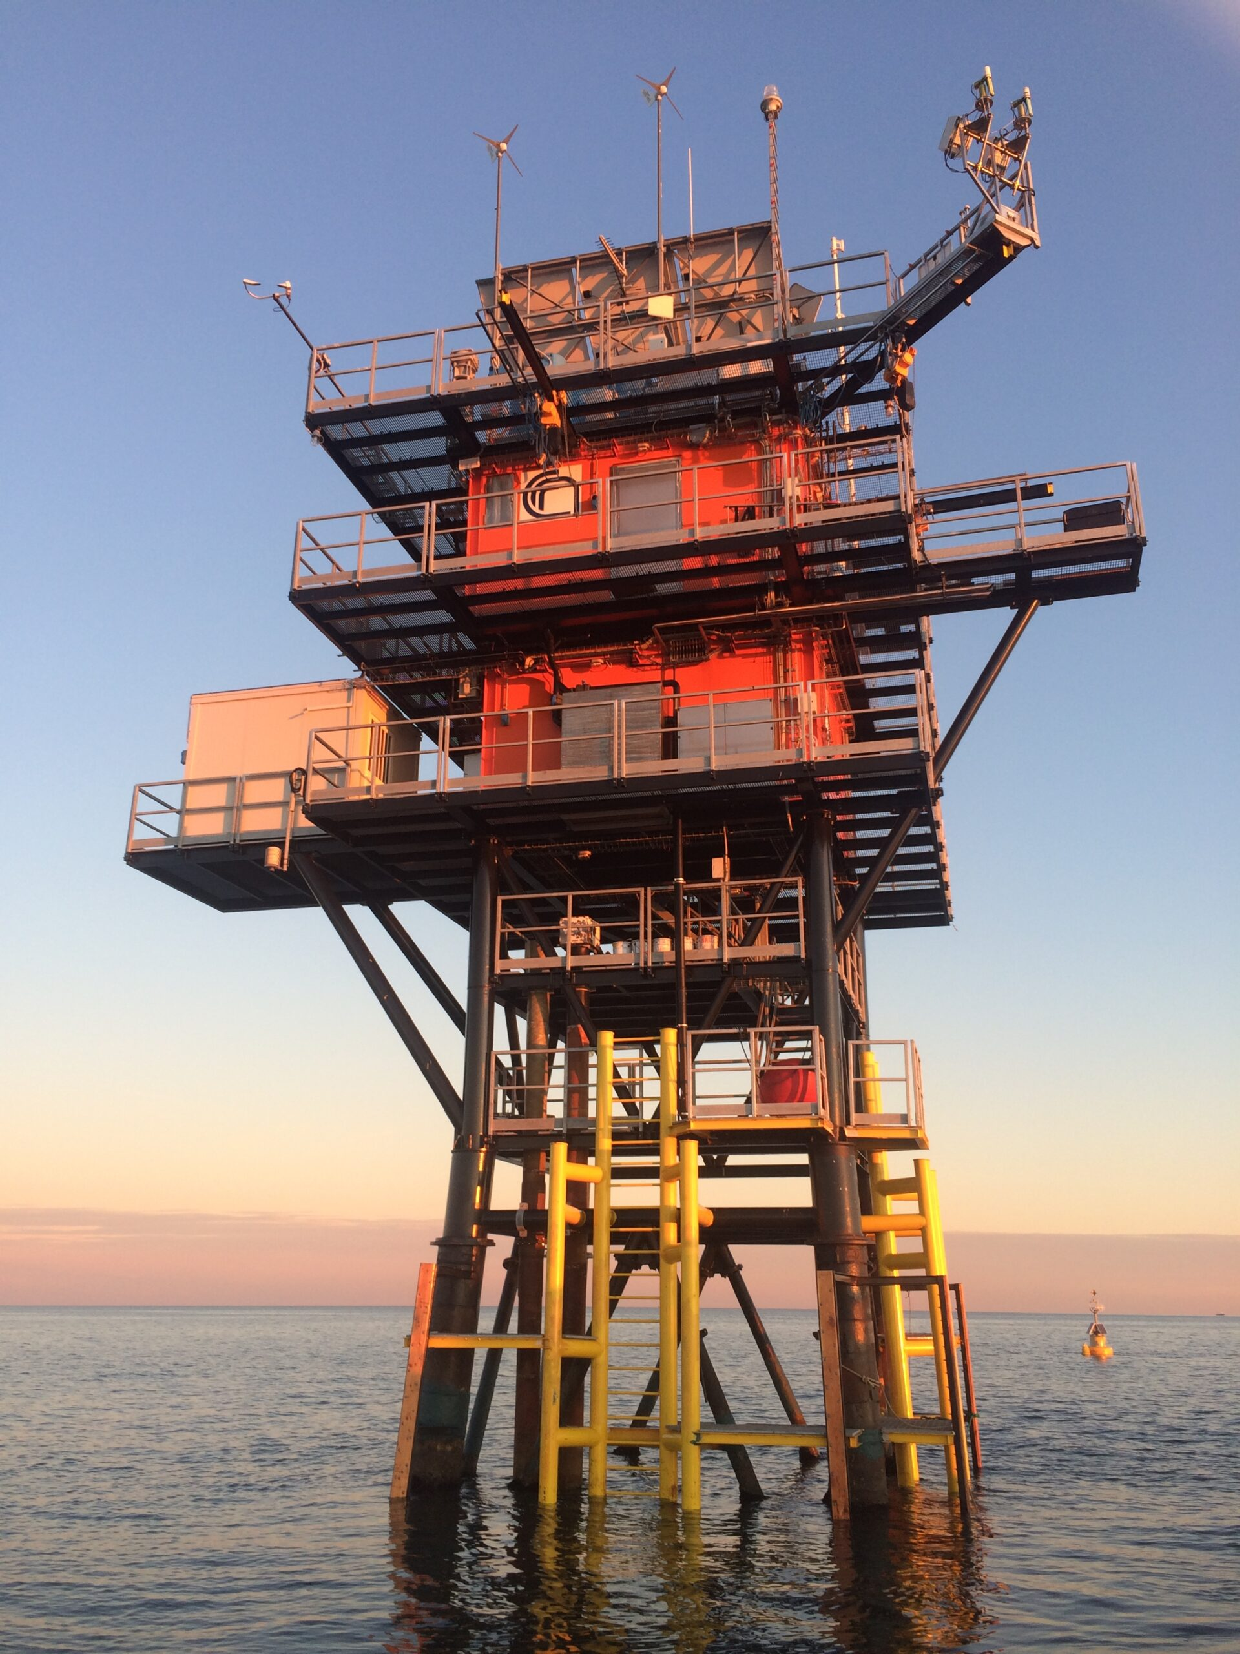
\includegraphics[width=\textwidth]{images/ifon_ptf_aaot.pdf}
\captionsetup{font=small, hypcap=false}
\captionof{figure}{Foto Piattaforma Oceanografica Acqua Alta\footcite[Fonte: ][\url{https://www.ismar.cnr.it/wp-content/uploads/2023/06/PTF-2018-05-Pomaro-1-scaled.pdf}]{website-ismar-cnr}.}
\label{fig:ifon_ptf_aaot}
\end{minipage}
\vspace{0.25cm}
\end{figure}

La Piattaforma Oceanografica \textbf{Acqua Alta} (vedi \autoref{fig:ifon_ptf_aaot}), installata nel 1970 a circa 10 miglia nautiche dal Lido di Venezia, alle coordinate: Lat. 45° 18.830' N, Lon. 12° 30.530' E, è una piattaforma dedicata esclusivamente alla ricerca oceanografica. Nella mappa in \autoref{fig:ifon_mappa_aaot} è possibile osservare la sua esatta posizione. La struttura è autonoma energicamente grazie a pannelli solari, generatori eolici e generatori diesel configurabili da remoto in modo da poter raccogliere dati continuativi nel tempo. I dati registrati dal sistema, in media ogni 30 minuti, vengono inviati a terra tramite collegamento wireless a banda larga e raccolti nel centro dati di ISMAR-VE (sede ISMAR di Venezia). Le variabili climatiche rilevate riguardano temperatura dell'aria, umidità, pressione, direzione e velocità del vento, precipitazioni e radiazione solare. L'elenco aggiornato delle variabili climatiche rilevate è disponibile nel sito di ISMAR-CNR\footcite[\url{https://www.ismar.cnr.it/infrastrutture/infrastrutture-oceanografiche/piattaforma-acqua-alta/}]{website-ismar-cnr}. Questo è possibile grazie ai sensori posti a 1.6 m (livello superficiale), 6 m (livello intermedio) e 14 m (livello di
fondo) di profondità\footcite[12-13]{rete-ifon}. Tra tutte le variabili climatiche, il cliente ha deciso che, per la prima versione dell'applicazione, si terrà conto solamente di 6 variabili (le uniche per le quali si è trovato il modo di accedere) osservate da diversi sensori:
\begin{enumerate}
    \item Direzione vento (sensore Davis Vantage PRO);
    \item Intensità vento (sensore Davis Vantage PRO);
    \item Direzione vento (sensore SIAP Micros t033 TDV);
    \item Intensità vento (sensore SIAP Micros t031 TDV);
    \item Altezza d'onda (sensore SIAP Micros t021 TLU16);
    \item Livello del mare (sensore SIAP Micros t039 TIDROM).
\end{enumerate}
Le prime due utilizzano l'\textbf{API allmeteo}, che si occupa di trasferire dati meteorologici, non in tempo reale, dal back-end allmeteo ai server di terze parti\footcite[\url{https://documenter.getpostman.com/view/11878734/TVYAf1Fn}]{website-api-allmeteo}, accessibili solo con autenticazione. Le altre utilizzano le \textbf{API del comune di Venezia}, accessibili tramite url TLS (\textit{Transport Layer Security protocol)} certificato con credenziali del tipo login/password. Un TLS è un protocollo progettato per consentire alle applicazioni client/server di comunicare su Internet senza intercettazioni, manomissioni o contraffazioni di messaggi\footcite[\url{https://foldoc.org/Transport_Layer_Security_protocol}]{website-TLS-def}. \par

% paloma
\begin{figure}[!ht]
\noindent\begin{minipage}{0.5\textwidth}
\vspace{1cm}
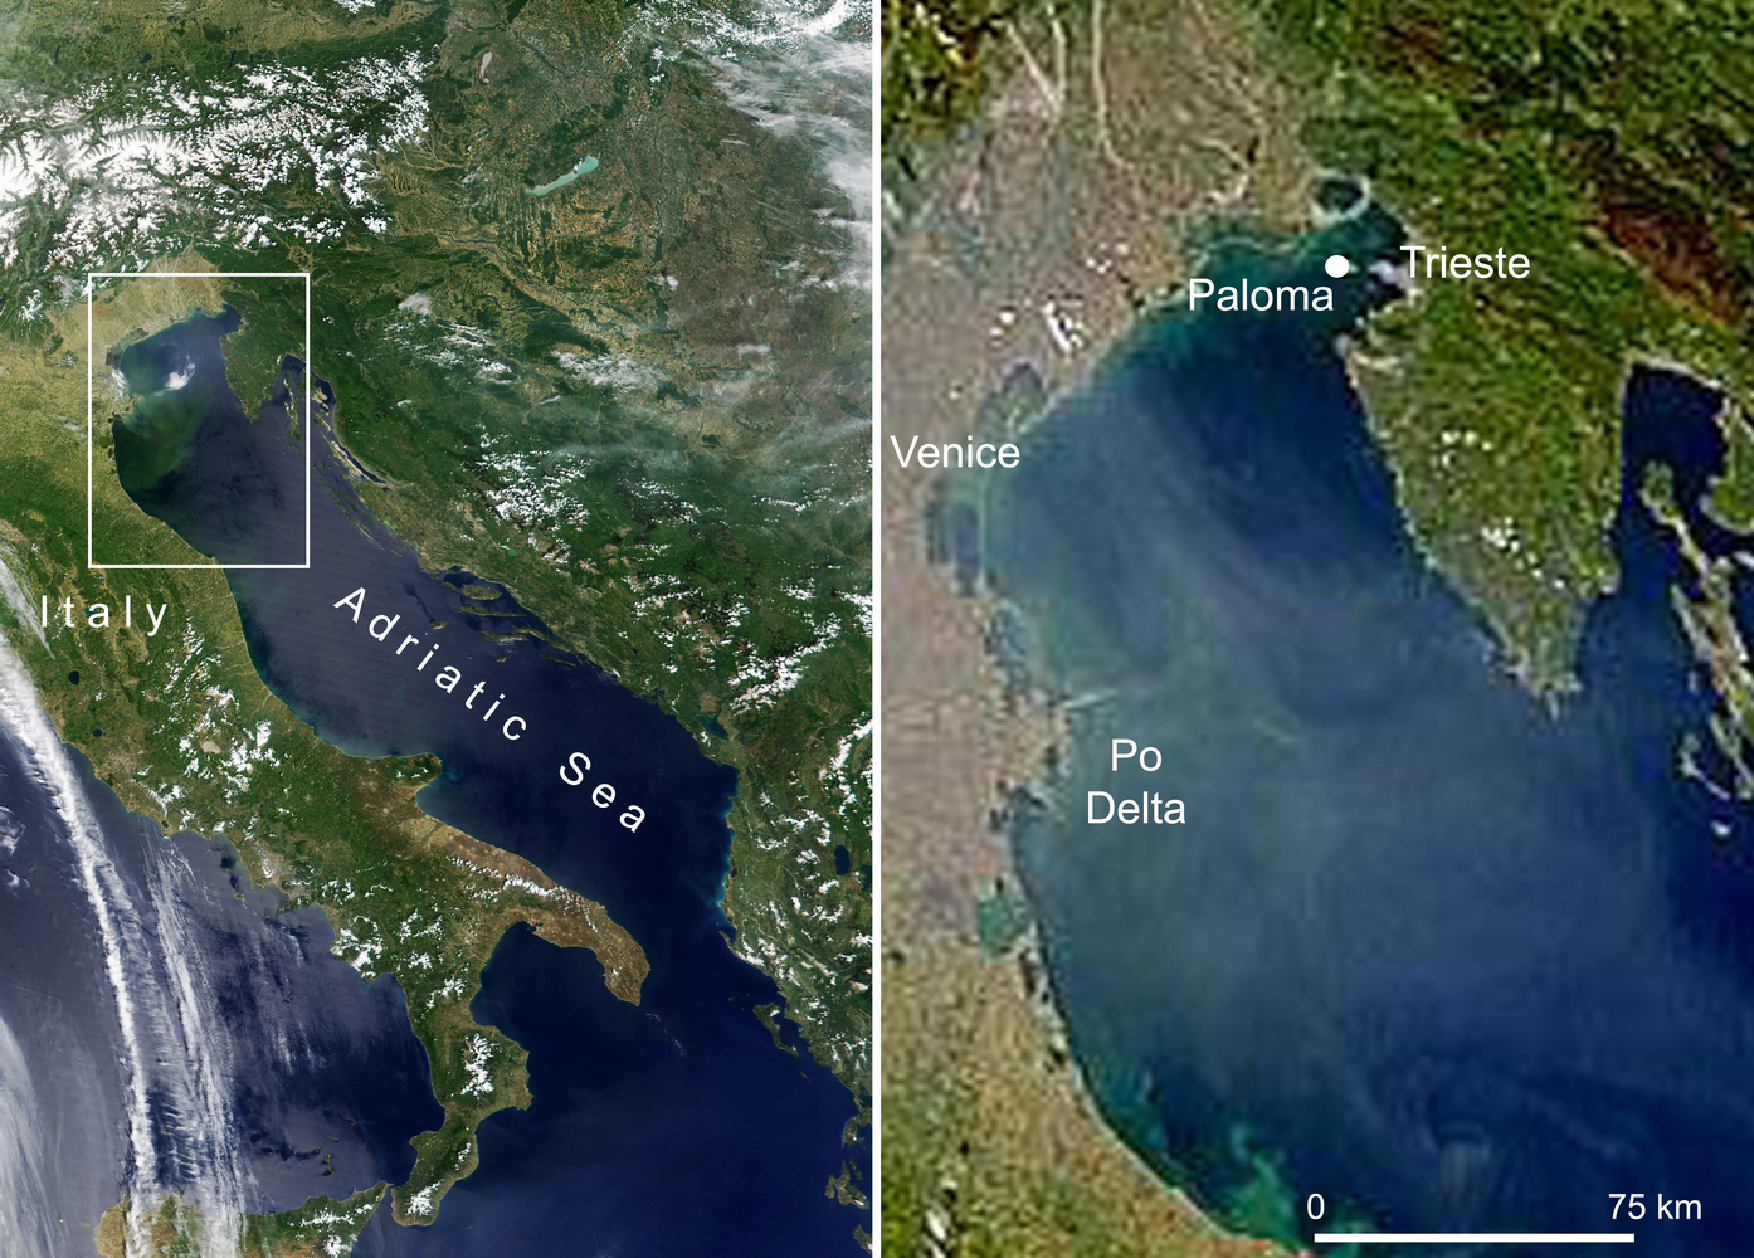
\includegraphics[width=\textwidth]{images/ifon_mappa_paloma.pdf}
\captionsetup{font=small, hypcap=false}
\captionof{figure}{Ubicazione meda Paloma\footcite[Fonte: ][\url{https://www.ismar.cnr.it/wp-content/uploads/2023/06/mappa-Paloma.pdf}]{website-ismar-cnr}.}
\label{fig:ifon_mappa_paloma}
\end{minipage}
\hspace{0.05\textwidth}
\begin{minipage}{0.4\textwidth}
\vspace{1cm}
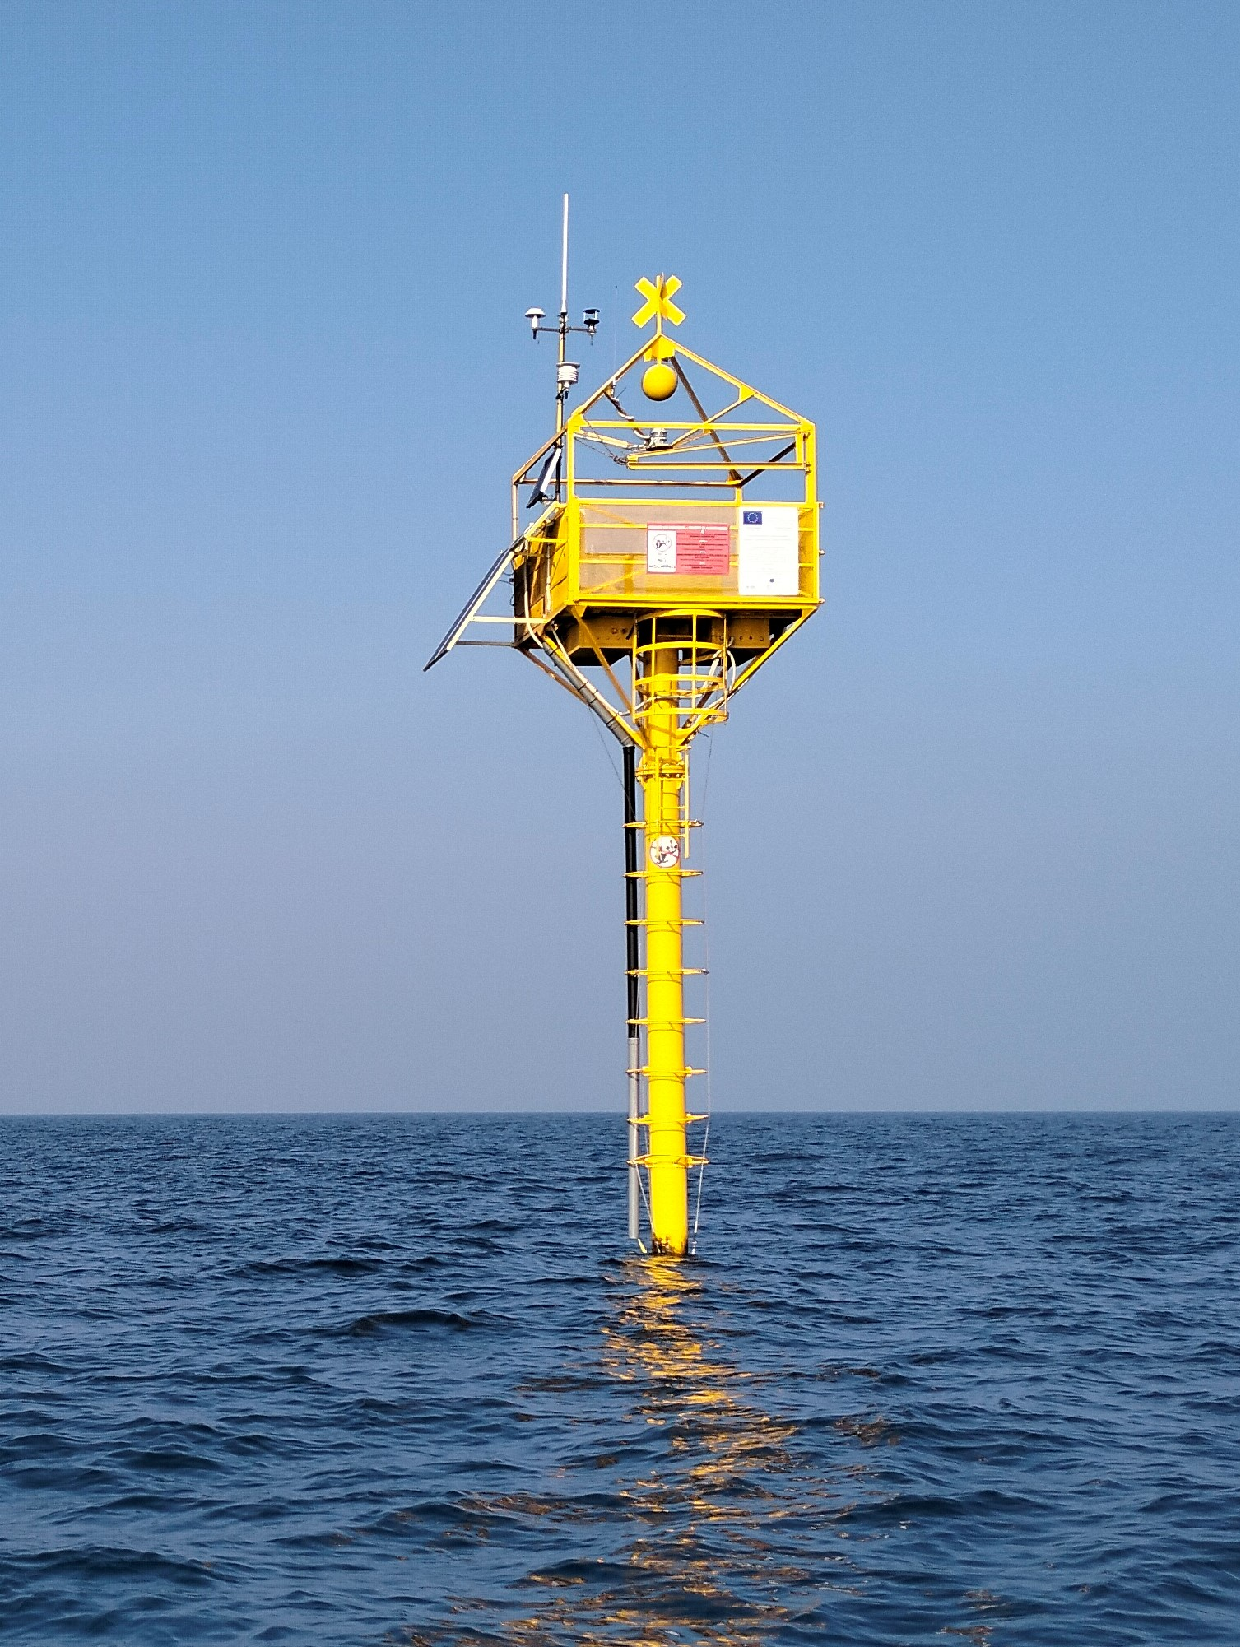
\includegraphics[width=\textwidth]{images/ifon_paloma.pdf}
\captionsetup{font=small, hypcap=false}
\captionof{figure}{Foto meda Paloma in mare\footcite[Fonte: ][\url{https://www.ismar.cnr.it/wp-content/uploads/2023/06/PALOMA_cantoni_01.pdf}]{website-ismar-cnr}.}
\label{fig:ifon_paloma}
\end{minipage}
\vspace{0.25cm}
\end{figure}

La meda\footnote{\textbf{méda} s. f. [voce settentr.: lat. mēta (v. mèta1)]. – 1. Nel linguaggio marin., propriam., nome di segnali disposti in mare, per lo più fissi, di forme e di colori varî, in metallo o in muratura, impiegati come avviso ai naviganti in corrispondenza di punti pericolosi (scogli affioranti, secche, ecc.), come punti di riferimento (per l’atterraggio, per l’imboccatura di un canale di accesso al porto, ecc.), per indicare, in acque ristrette, il tratto di mare navigabile con sicurezza: m. luminosa, quella sormontata da un fanale, generalmente rosso o verde, e dipinta dello stesso colore; m. semielastica, specie di boa, generalmente luminosa, ancorata al fondo del mare per mezzo di una robusta asta di ormeggio, in grado di galleggiare e di oscillare (anche verticalmente) per mantenere visibile il segnale in presenza di onde alte sino a tre metri; m. sonora, fornita di trasmettitore acustico (nautofono, ecc.); \cite{treccani-meda}.} \textbf{PALOMA} -- \textit{Piattaforma Avanzata Laboratorio Oceanografico Mare Adriatico} -- (vedi \autoref{fig:ifon_paloma}) si trova, come si può notare in \autoref{fig:ifon_mappa_paloma}, al centro del Golfo di Trieste, a circa 8 miglia nautiche dalla costa triestina, su un fondale di 25 metri. È operativa dal 2002, e da allora fornisce dati meteo marini raccolti ogni 5 minuti e trasmessi a terra ogni 3 ore. I parametri meteorologici, misurati tramite sensori posti a 3, 15 e 14 metri di profondità, includono la temperatura, l’umidità, la pressione, le precipitazioni, la direzione e intensità del vento e la radiazione solare. Inoltre, a 3m di profondità viene misurato l'ossigeno disciolto. L'elenco aggiornato delle variabili climatiche rilevate è disponibile nel sito di ISMAR-CNR\footcite[\url{https://www.ismar.cnr.it/infrastrutture/infrastrutture-oceanografiche/paloma/}]{website-ismar-cnr}. I dati acquisiti vengono trasmessi regolarmente ad un server dedicato presso la sede di ISMAR-TS (sede ISMAR di Trieste)\footcite[11-12]{rete-ifon}.\par

% meda s1-gb
\begin{figure}[!ht]
\noindent\begin{minipage}{0.5\textwidth}
\vspace{1cm}
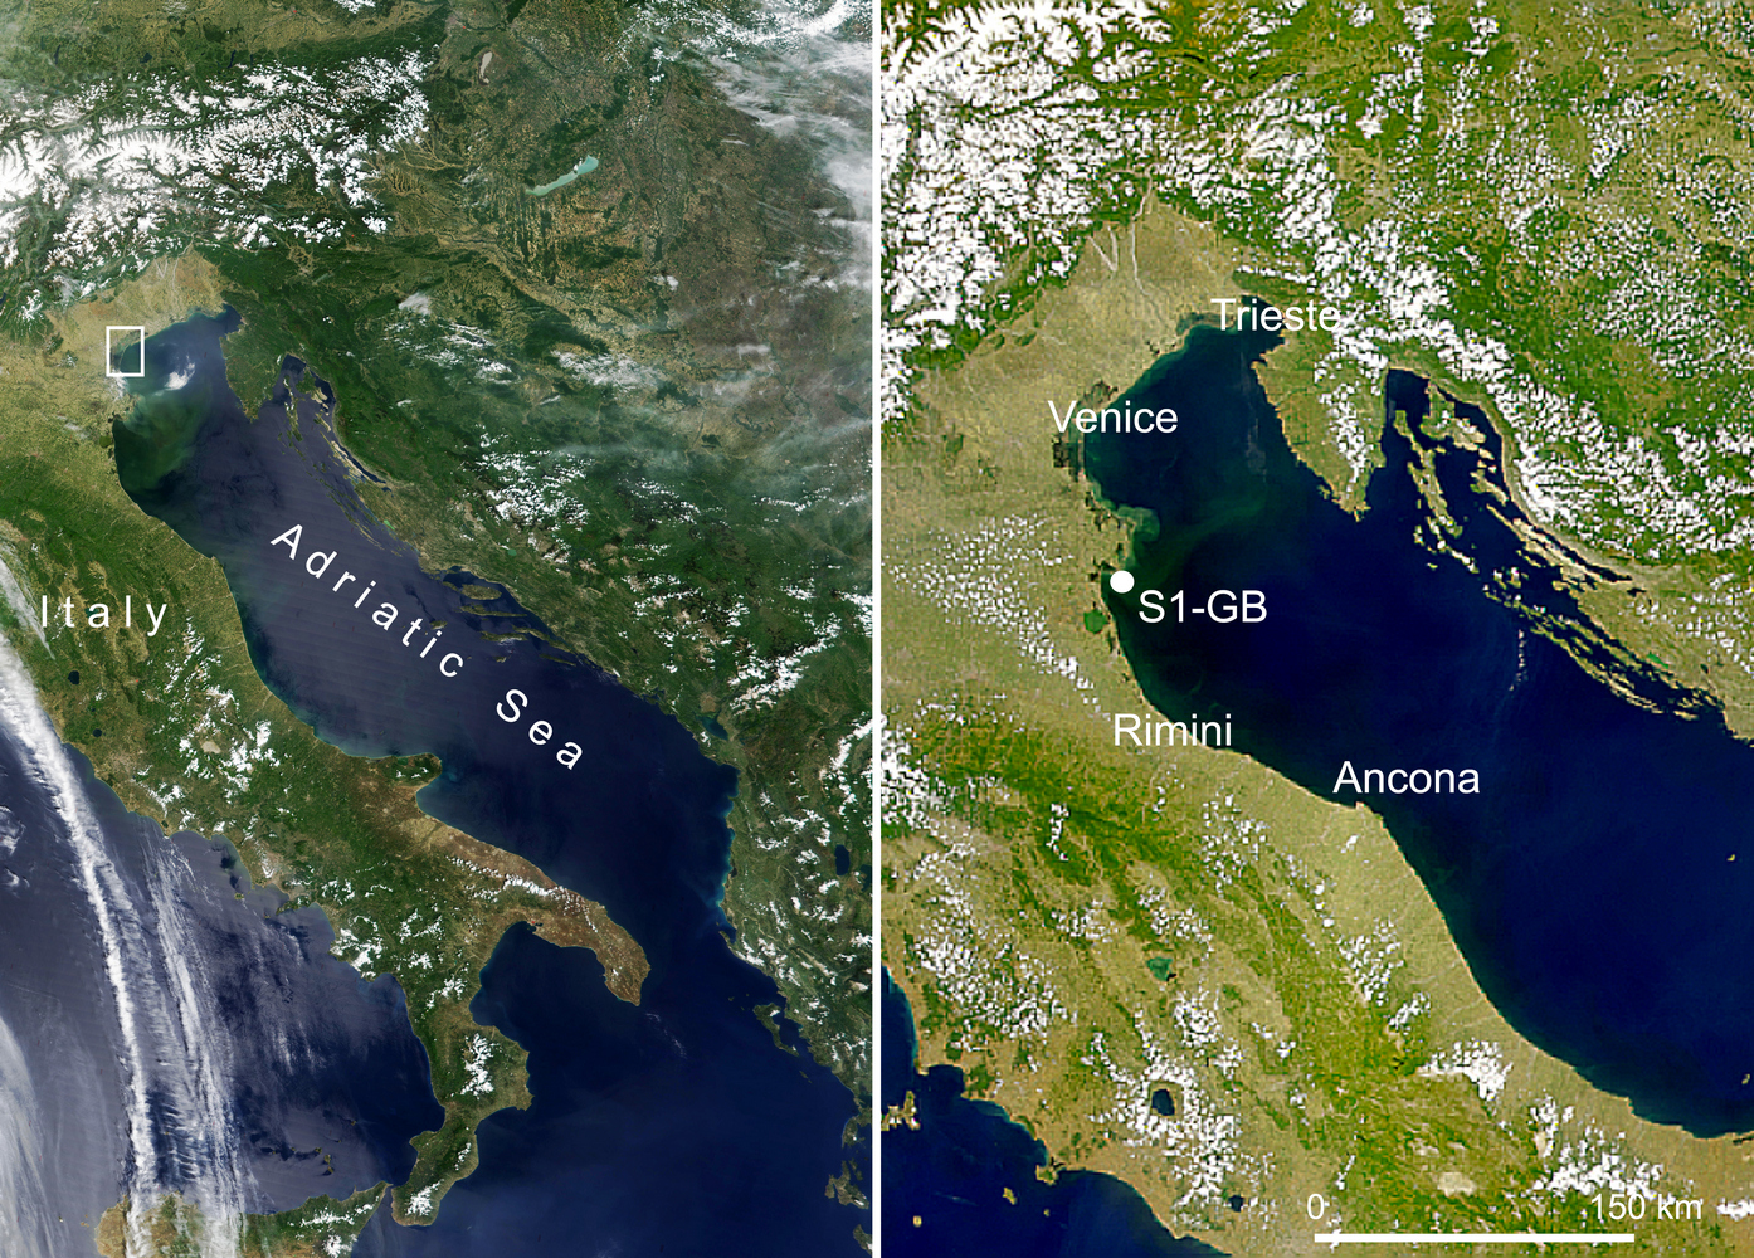
\includegraphics[width=\textwidth]{images/ifon_mappa_s1gb.pdf}
\captionsetup{font=small, hypcap=false}
\captionof{figure}{Posizione meda S1-GB\footcite[Fonte: ][\url{https://www.ismar.cnr.it/wp-content/uploads/2023/06/mappa-S-GB.pdf}]{website-ismar-cnr}.}
\label{fig:ifon_mappa_s1gb}
\end{minipage}
\hspace{0.05\textwidth}
\begin{minipage}{0.4\textwidth}
\vspace{1cm}
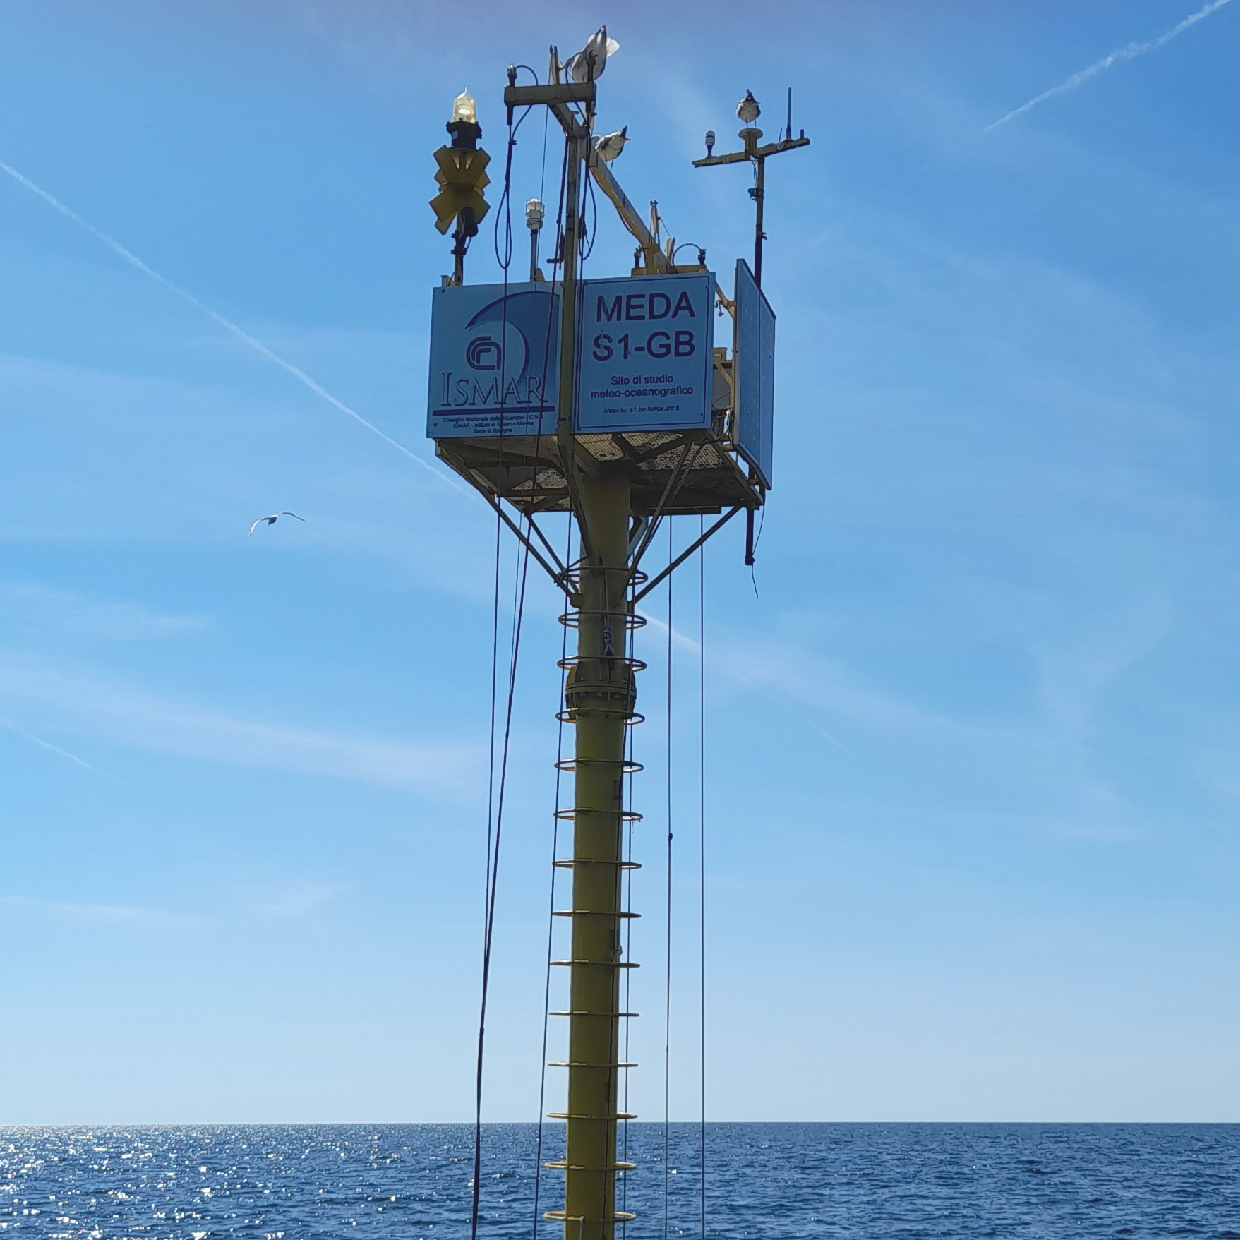
\includegraphics[width=\textwidth]{images/ifon_s1gb.pdf}
\captionsetup{font=small, hypcap=false}
\captionof{figure}{Foto meda S1-GB\footcite[Fonte: ][\url{https://www.ismar.cnr.it/wp-content/uploads/2023/06/S1-GB_Foto1_cr1.pdf}]{website-ismar-cnr}.}
\label{fig:ifon_s1gb}
\end{minipage}
\vspace{0.25cm}
\end{figure}

La \textbf{meda S1-GB} (vedi \autoref{fig:ifon_s1gb}) è situata alle coordinate Lat. 44° 44.4' N, Lon. 12 27.3' E, a circa 4 miglia nautiche a Sud della foce di Po di Goro (Delta del fiume Po - Adriatico Settentrionale, vedi \autoref{fig:ifon_mappa_s1gb}), su di un fondale di 22.5 m. Nasce come \textit{boa S1} nel 2004, per poi essere potenziata sostituendo la boa galleggiante con una stazione fissa a meda elastica. L'elasticità fa in modo che quando avviene una collisione la meda si inclini momentaneamente per poi ritornare in posizione, riducendo i possibili danni dovuti allo scontro tra meda e veicolo marino\footcite[1-4]{resinex-meda-elastica} (in \autoref{fig:boa_vs_medaelastica} è possibile osservare il confronto tra boa fissa e meda elastica). Da qui il nome meda S1-GB (\textit{già Boa} meteo-oceanografica S1). Essa è costituita da vari sensori posti a diversi livelli che acquisiscono parametri oceanografici, meteorologici e biogeochimici\footcite[13-15]{rete-ifon}. In particolare contiene la strumentazione oceanografica a due livelli di profondità, -2,5 m e -18,5 m. Le variabili analizzate riguardano la temperatura della superficie del mare, l'ossigeno disciolto, la clorofilla e così via. Esse sono ampiamente descritte nel sito di ISMAR-CNR\footcite[Fonte: ][\url{https://www.ismar.cnr.it/infrastrutture/infrastrutture-oceanografiche/meda-s1-gb/}]{website-ismar-cnr}.\par

\begin{figure}[!ht]
\noindent\begin{minipage}{0.5\textwidth}
\vspace{1cm}
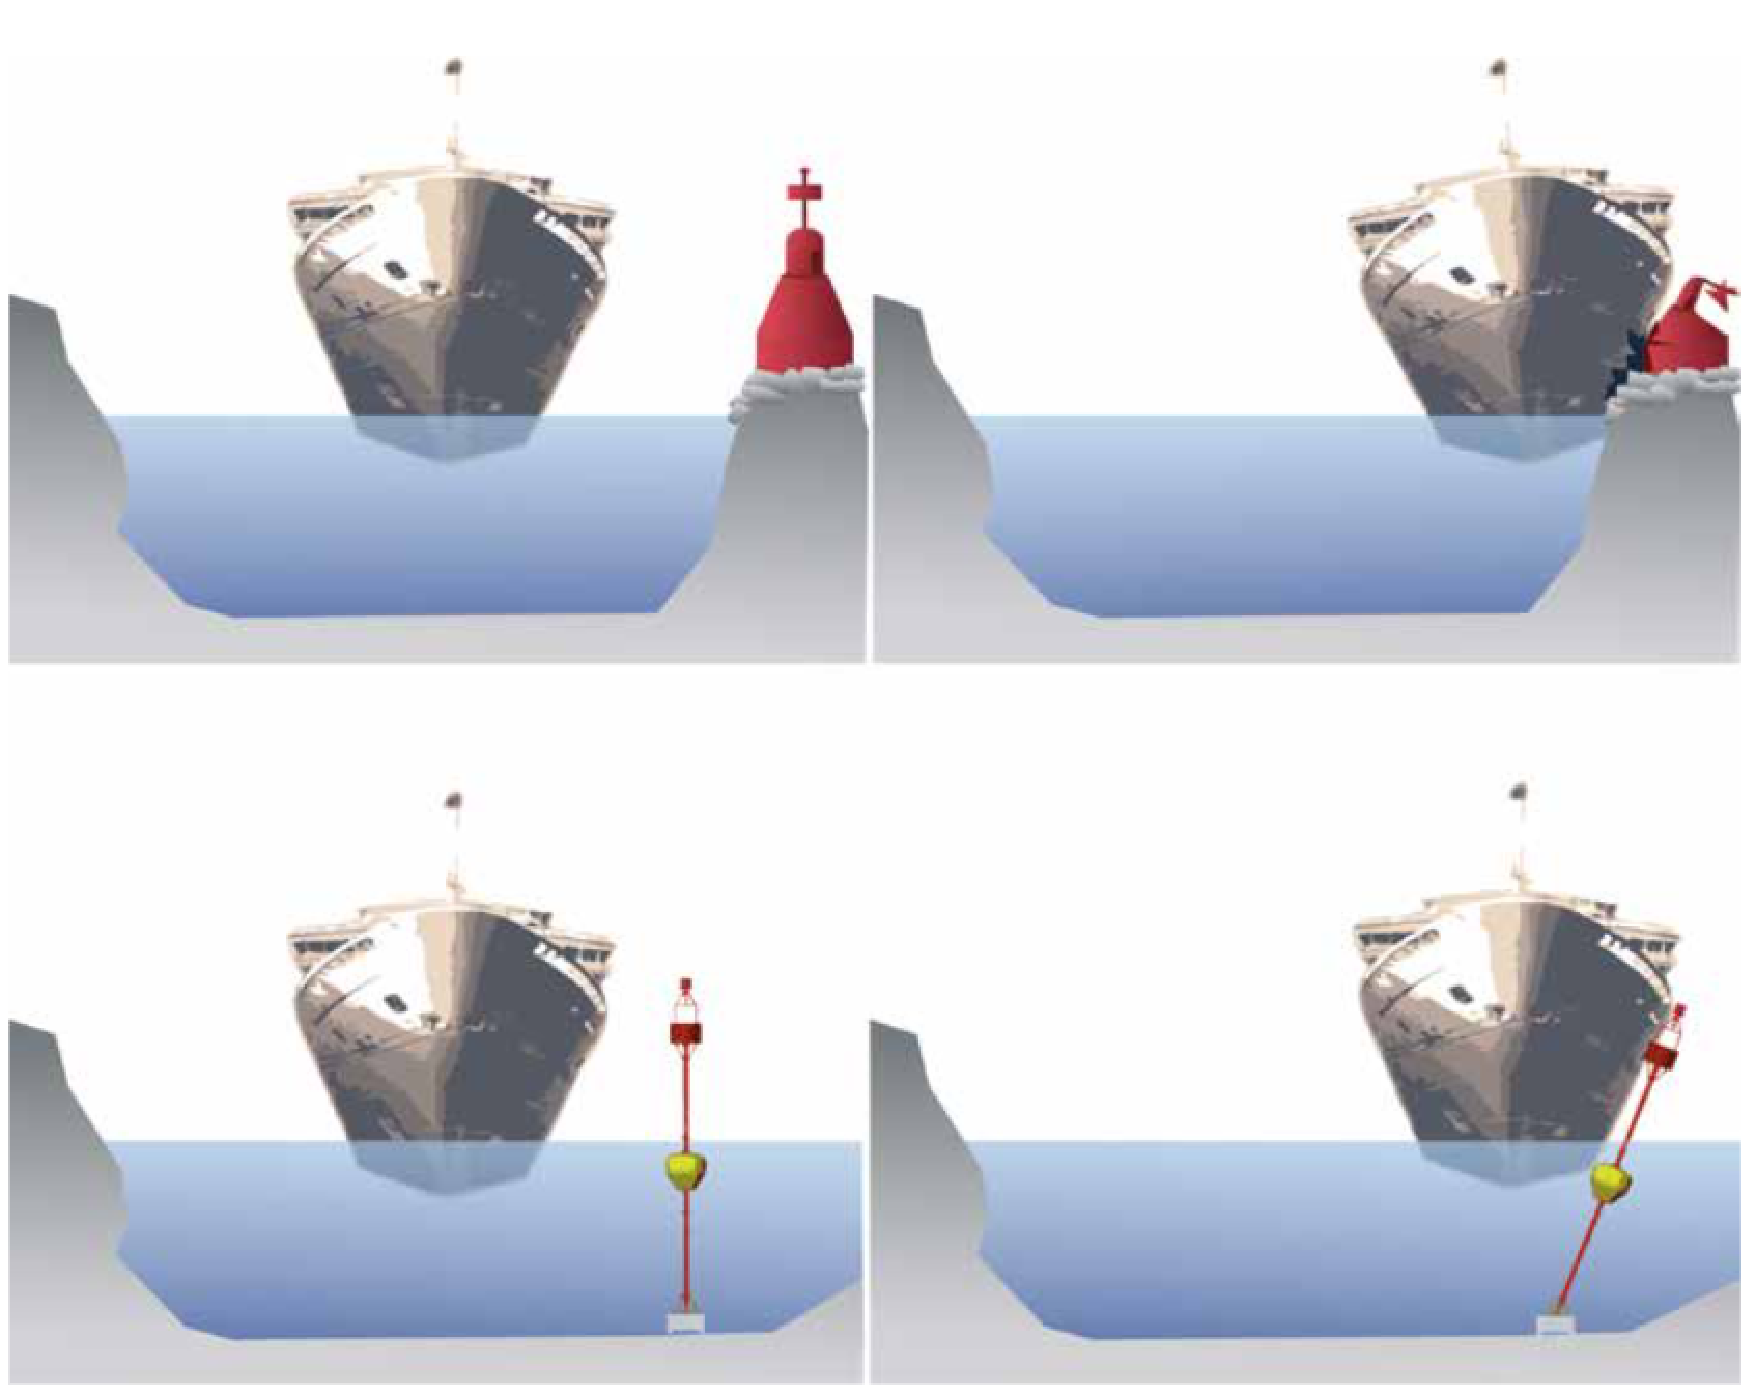
\includegraphics[width=\textwidth]{images/boa_vs_medaelastica.pdf}
\captionsetup{font=small, hypcap=false}
\captionof{figure}{Confronto tra classica boa fissa (in alto) e innovativa meda elastica (in basso)\footcite[Fonte: ][4]{resinex-meda-elastica}.}
\label{fig:boa_vs_medaelastica}
\end{minipage}
\hspace{0.05\textwidth}
\begin{minipage}{0.4\textwidth}
\begin{small}
Disegno che evidenzia il principale vantaggio di una meda elastica: evitare danni nonostante le collisioni. Questo vale sia per la meda che per il veicolo con cui avviene lo scontro. Un'ulteriore nota positiva riguarda la facilità di trasferimento nel caso in cui ci sia necessità di spostarla.
\end{small}
\end{minipage}
\vspace{0.25cm}
\end{figure} 

% boa e1
\begin{figure}[!ht]
\noindent\begin{minipage}{0.5\textwidth}
\vspace{1cm}
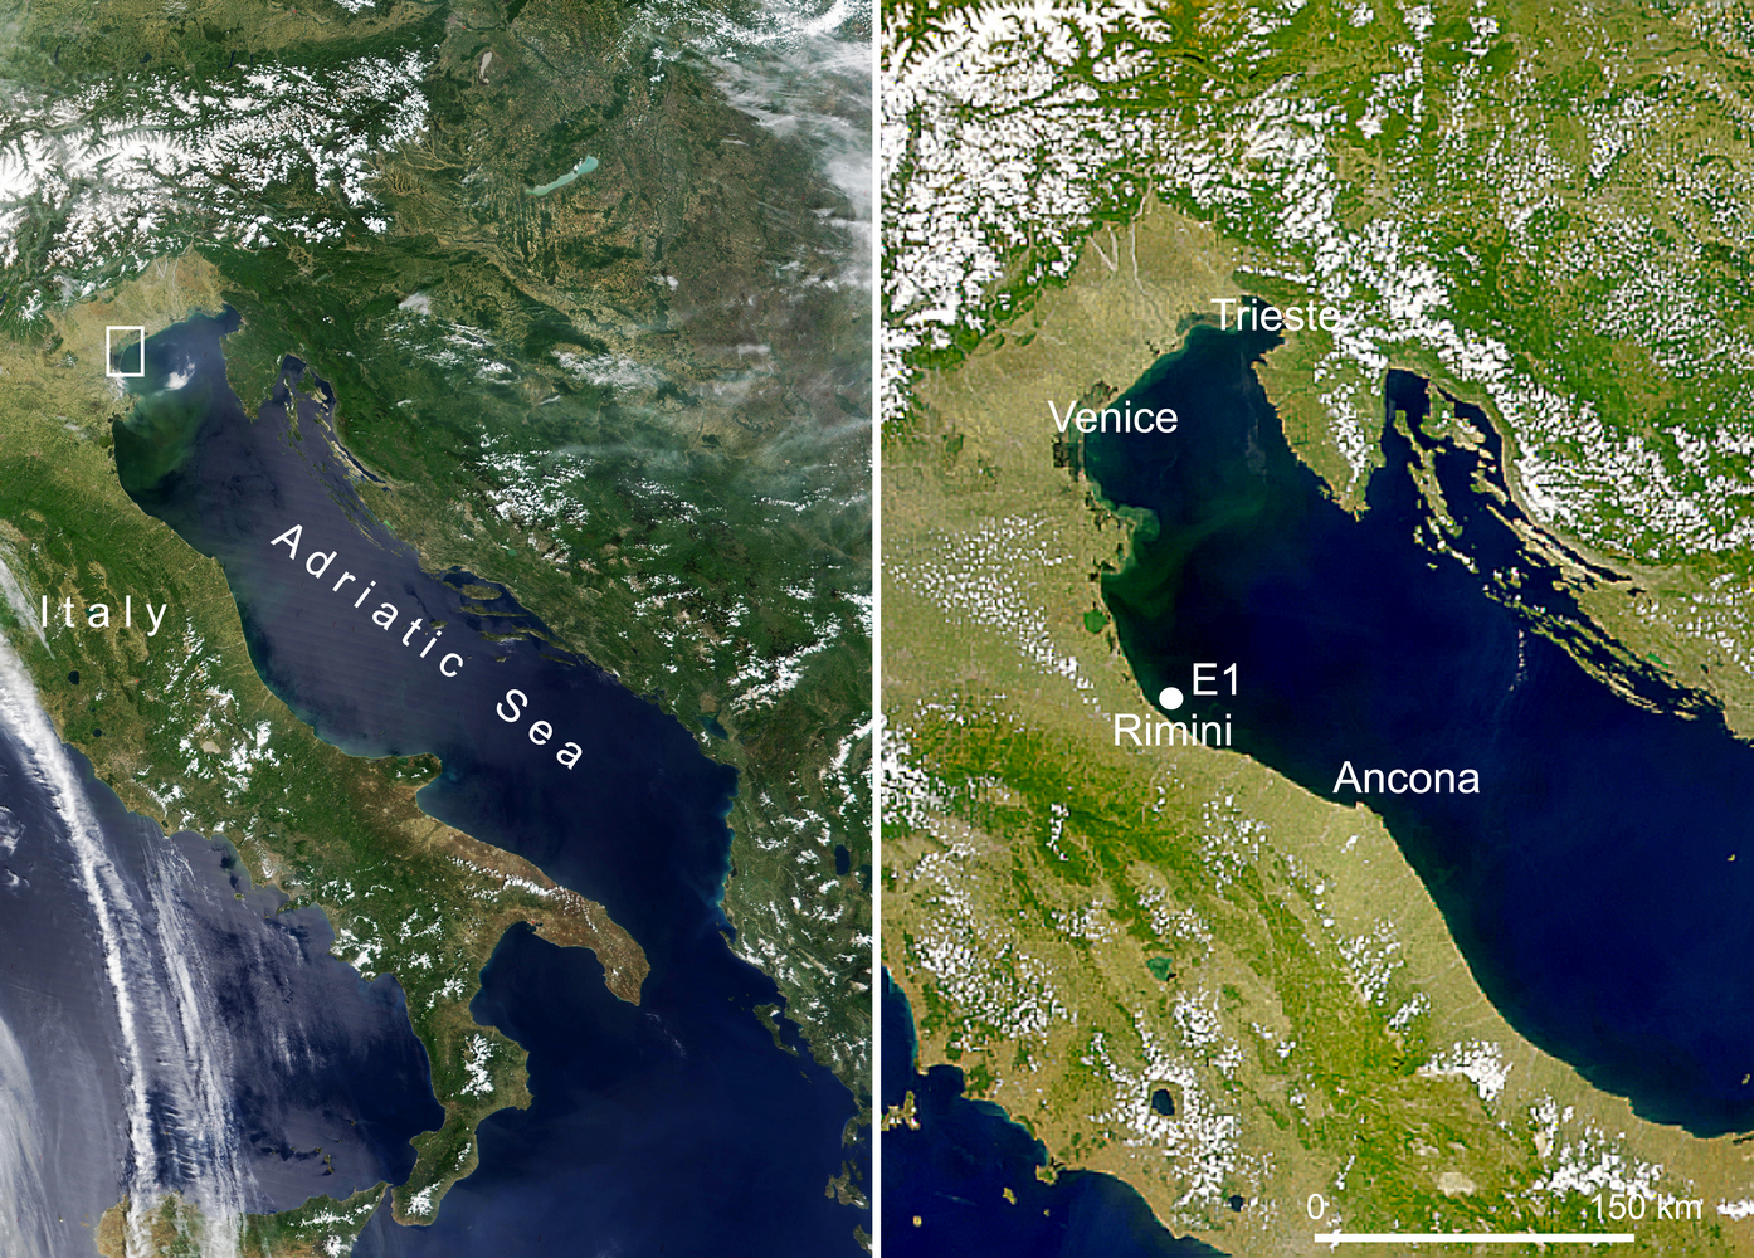
\includegraphics[width=\textwidth]{images/ifon_mappa_boa_e1.pdf}
\captionsetup{font=small, hypcap=false}
\captionof{figure}{Posizione boa E1\footcite[Fonte: ][\url{https://www.ismar.cnr.it/wp-content/uploads/2023/06/mappa-E1.pdf}]{website-ismar-cnr}.}
\label{fig:ifon_mappa_boa_e1}
\end{minipage}
\hspace{0.05\textwidth}
\begin{minipage}{0.4\textwidth}
\vspace{1cm}
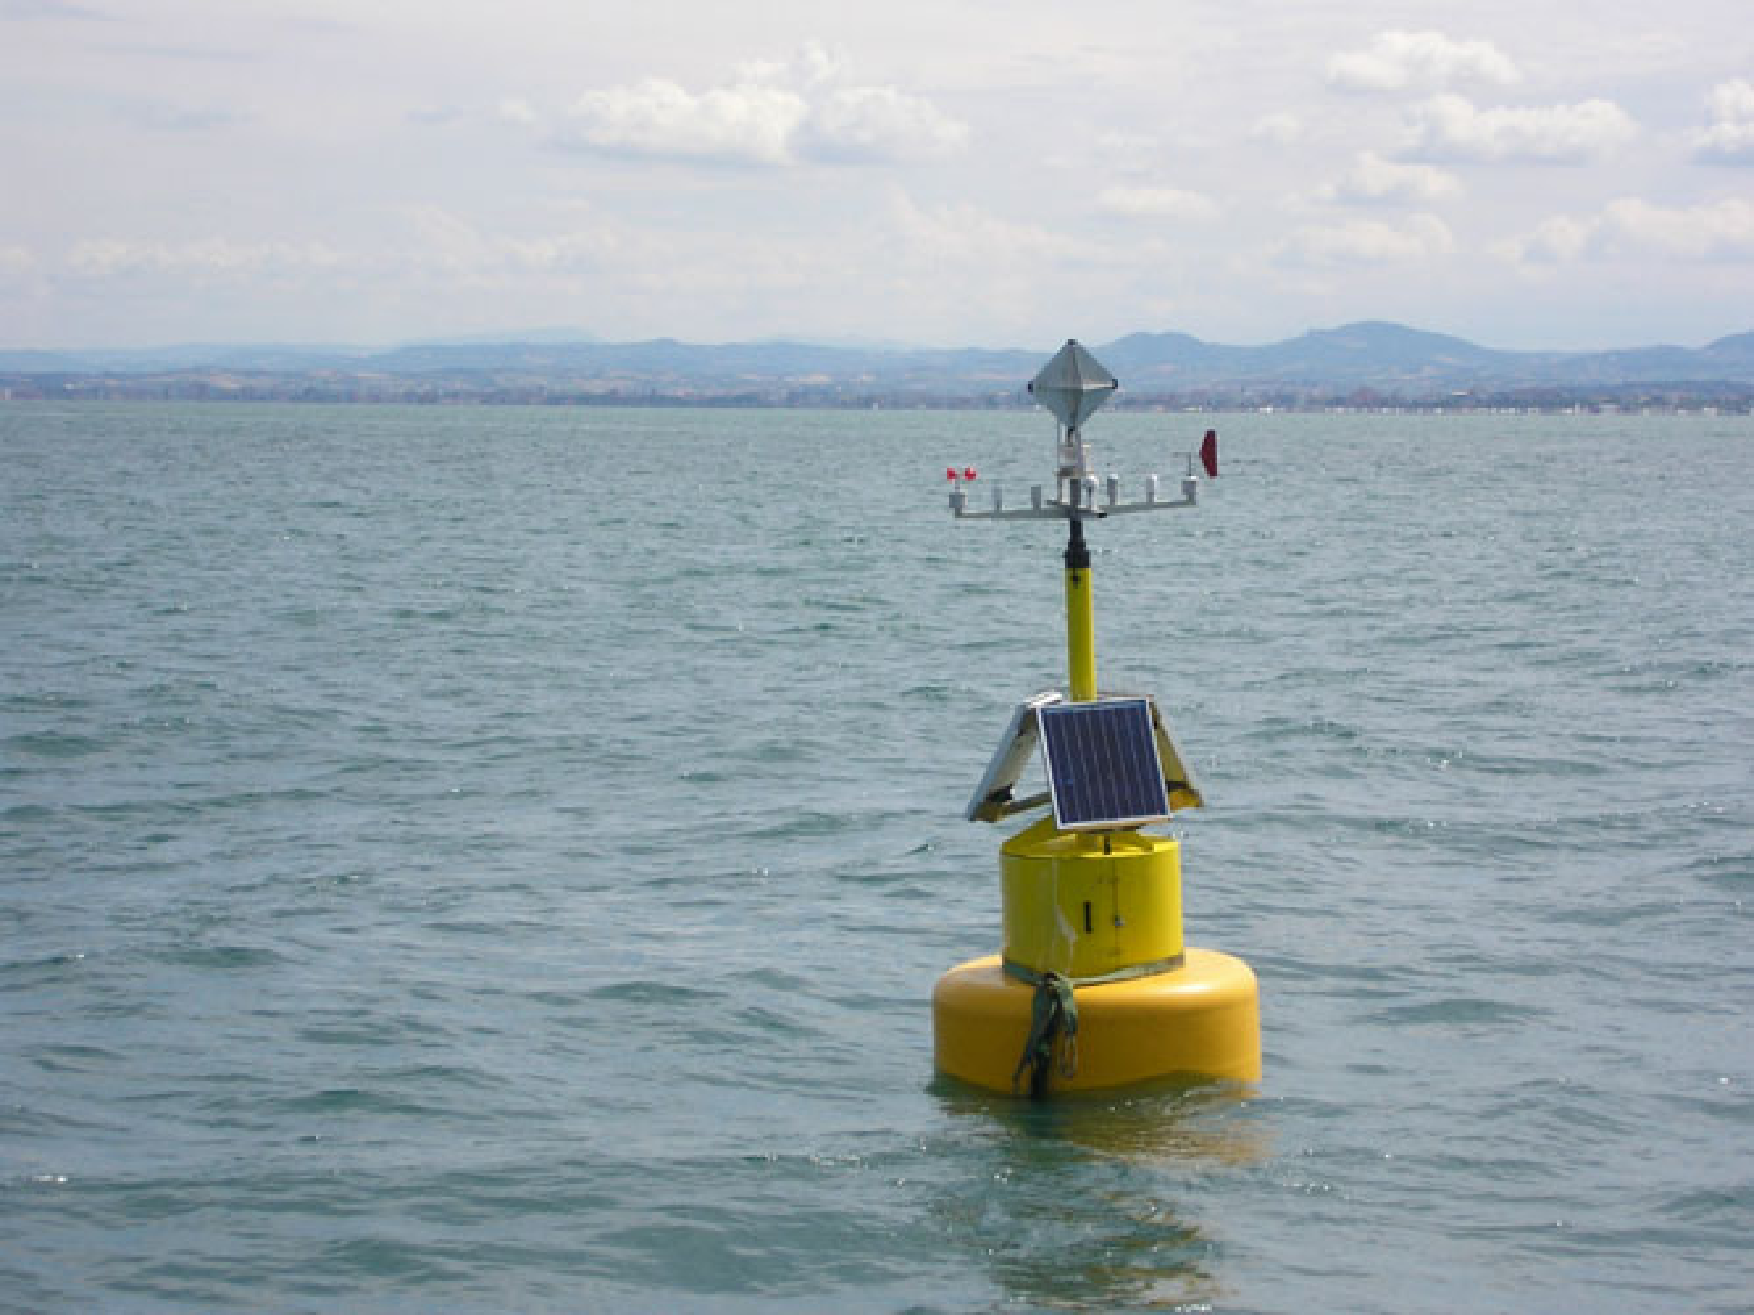
\includegraphics[width=\textwidth]{images/ifon_boa_e1.pdf}
\captionsetup{font=small, hypcap=false}
\captionof{figure}{Foto boa E1\footcite[Fonte: ][\url{https://www.ismar.cnr.it/wp-content/uploads/2022/11/boe-costa-romagnola-ismar-cnr-2.pdf}]{website-ismar-cnr}.}
\label{fig:ifon_boa_e1}
\end{minipage}
\vspace{0.25cm}
\end{figure}

La \textbf{boa meteo-oceanografica E1} si trova nell'Adriatico Settentrionale, a circa 4 miglia nautiche a Nord della città di Rimini. Il sistema è ancorato al fondo mare mediante catena e corpo morto su di un fondale di 10.5 m. Si trova alle coordinate Lat. 44 08.5' N, Lon. 12 34.2' E dal 2006 (vedi \autoref{fig:ifon_mappa_boa_e1} e \autoref{fig:ifon_boa_e1}). Essa è dotata di strumentazione per il rilevamento di parametri meteorologici a 2.5m sul livello del mare e parametri oceanografici su due livelli di sensori  installati alle profondità di 1.6m
(livello superficiale) e 8m (livello profondo). Le variabili oceanografiche a 8m riguardano salinità, temperatura del mare e ossigeno disciolto, mentre in superficie viene misurata la clorofilla e la torbidità. Esse sono descritte nel sito di ISMAR-CNR\footcite[\url{https://www.ismar.cnr.it/infrastrutture/infrastrutture-oceanografiche/boa-e1/}]{website-ismar-cnr}.\par

I dati di queste ultime tre stazioni (Paloma, S1-GB ed E1) non sono pubblici e, nonostante i tentavi di cercare una soluzione al problema, non è stato fornito l'accesso a nessuna variabile misurata.\par

% RADAR 
\paragraph{Radar.}
Il \textit{radar ad alta frequenza} (\textbf{HFR}) è uno strumento di telerilevamento terrestre che permette di ottenere misurazioni su correnti, onde e direzione dei venti\footcite[2]{10.3389/fmars.2017.00008}.
I radar sono in grado di fornire mappe di velocità superficiale in ampie regioni del mare (range fino a 200km) ad intervalli di tempo regolari, tipicamente di un’ora, consentendo il monitoraggio continuo delle correnti marine superficiali\footcite[\url{https://www.ismar.cnr.it/infrastrutture/infrastrutture-oceanografiche/rete-radar-costiera/}]{website-ismar-cnr}.

%\paragraph{Rete HFR-TirLig.} 
La rete radar \textbf{HFR-TirLig} di ISMAR-CNR fornisce accesso ai dati in tempo reale provenienti dalle stazioni attive lungo la costa del Mar Tirreno nordoccidentale e Mar Ligure (vedi \autoref{fig:radar_map}). La rete è composta da due stazioni che emettono a frequenze di 13,5 MHz e due che emettono a frequenze di 16,275 MHz, fornendo dati orari di corrente radiale (\textit{singole misurazioni per ogni stazione}) con una risoluzione di portata rispettivamente di 1,5 km e 1 km e una copertura radiale prossima rispettivamente a 80 km e 40 km. Le misurazioni radiali delle singole stazioni vengono combinate su una griglia regolare, con risoluzione spaziale di 2km, su una copertura totale di circa 9000 km quadrati, al fine di ottenere le misurazioni totali. I dati radiali sono misurazioni effettuate per ogni singolo radar, mentre i dati totali rappresentano l'unione, tramite apposite tecniche, dei dati radiali (come se fossero dati di un unico radar). In questo modo i dati saranno meno precisi ma comunque validi\footcite[\url{https://www.hfrnode.eu/networks/hfr-tirlig/}]{website-hfr-tirlig}.

% img radar position on map %
\begin{figure}[!ht]
\noindent\begin{minipage}{0.5\textwidth}
\vspace{1cm}
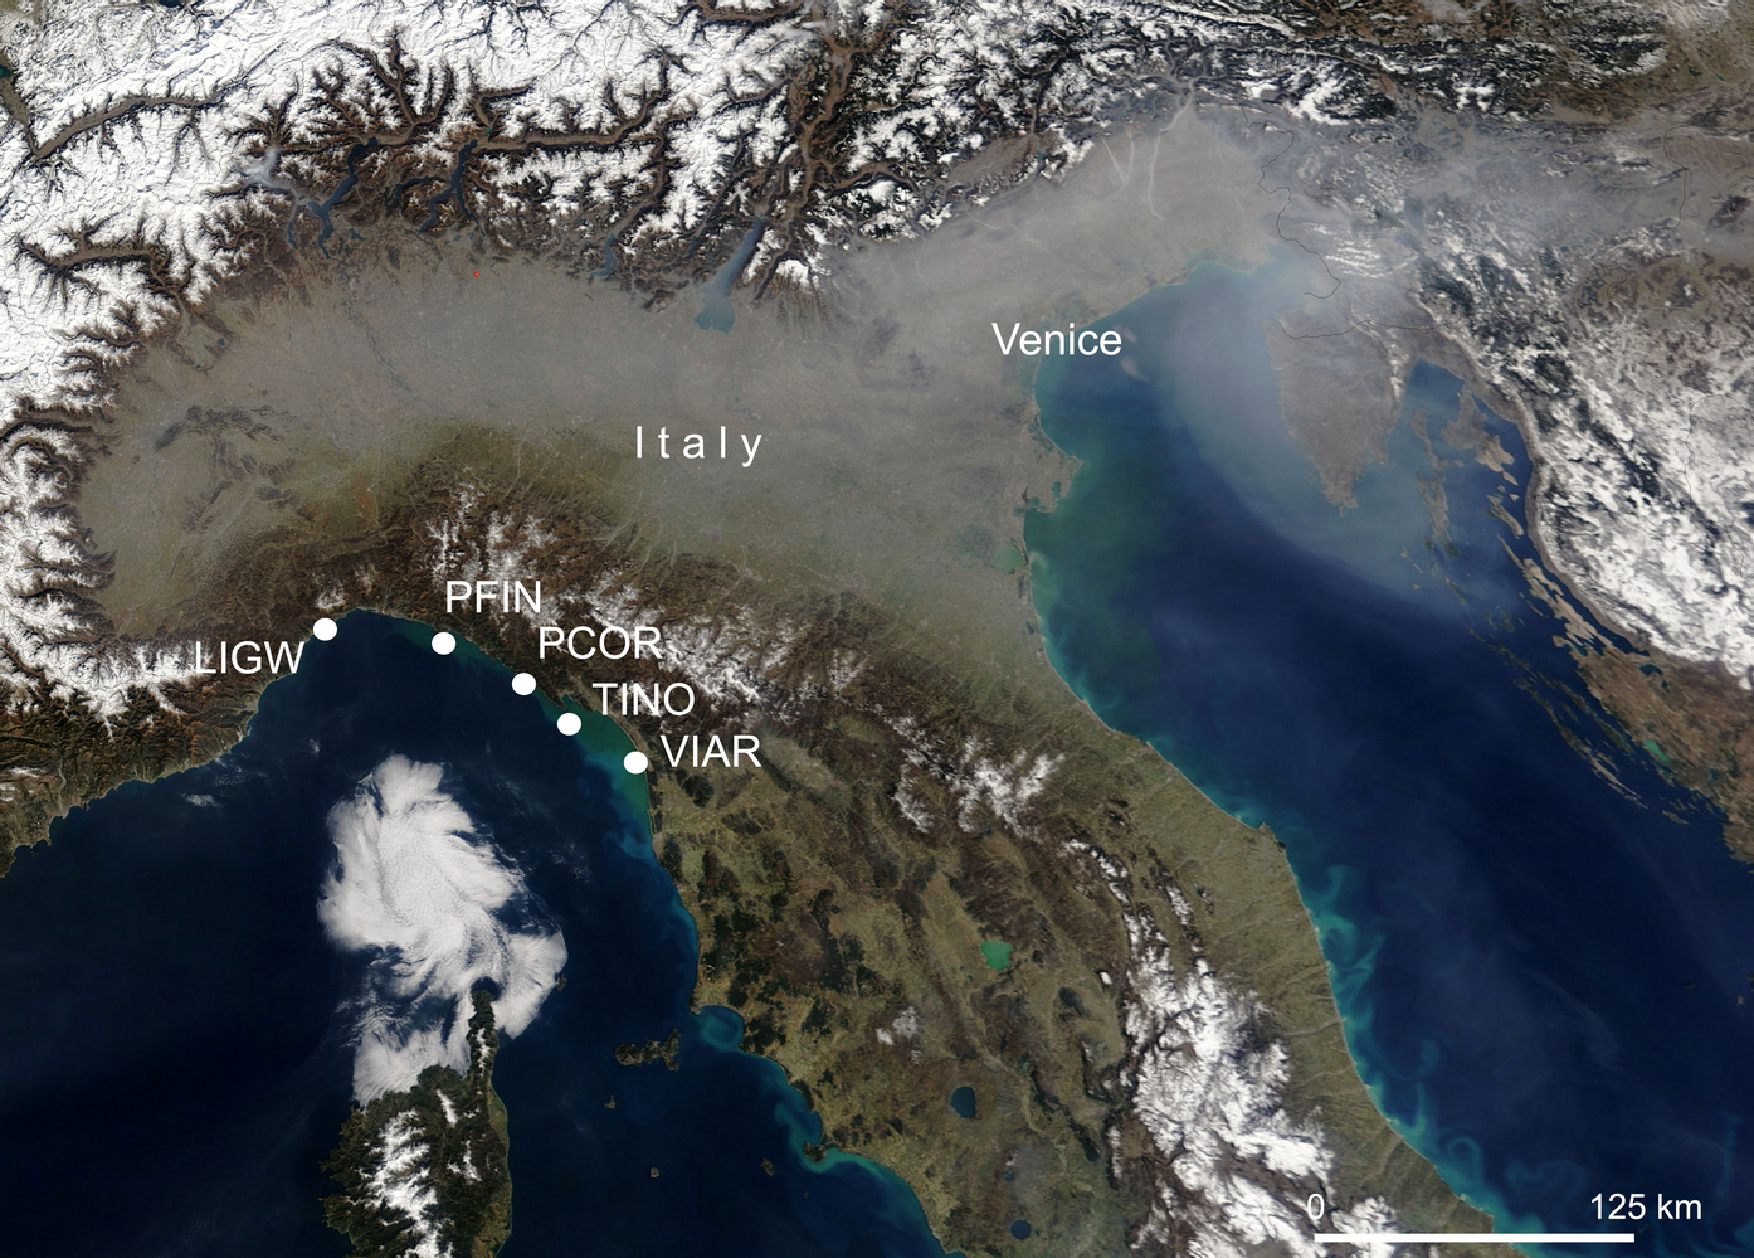
\includegraphics[width=\textwidth]{images/radar_map.pdf}
\captionsetup{font=small, hypcap=false}
\captionof{figure}{Rete radar ad alta frequenza (\textit{HF=High Frequency})\footcite[Fonte: ][\url{https://www.ismar.cnr.it/wp-content/uploads/2023/06/mappa-Radar-HF.pdf}]{img-map-radar-hf}.}
\label{fig:radar_map}
\end{minipage}
\hspace{0.05\textwidth}
\begin{minipage}{0.4\textwidth}
\begin{small}
LIGW: Celle Ligure (SV) 4.2987139 N, 9.21837778 E.\\PCOR: Monterosso al Mare (SP) 44.1433333 N, 9.65944 E.\\TINO: Isola del Tino (SP) 44.0263889 N, 9.849166667 E.\\PFIN: Portofino (GE) 44.2986111 N, 9.218333334 E.\\VIAR: Viareggio (LU) 43.8580556 N, 10.237222222 E.
\end{small}
\end{minipage}
\vspace{0.25cm}
\end{figure}

%\paragraph{Misurazioni.} 
I dati sono disponibili in un catalogo THREDDS\footcite[\url{https://thredds.hfrnode.eu:8443/thredds/NRTcurrent/HFR-TirLig/HFR-TirLig_catalog.html}]{thredds-hfr-trilig} aggiornato contenente le variabili osservate in formato standard NetCDF-4\footcite[19-47]{HFR_QC_JERICO}.
\vspace{0.25cm}

\begin{quote}
\textit{I cataloghi THREDDS sono documenti XML, forniti dal THREDDS Data Server (TDS)\footcite[\url{https://doi.org/10.5065/D6N014KG}]{website-unidata-ucar-edu}, che elencano i set di dati e i servizi -- \textit{protocolli} -- per l'accesso ad essi.}
\end{quote}

Come accennato nel paragrafo precedente, le misurazioni si distinguono in totali e radiali. Al momento, dato che l'applicazione si rivolge a un pubblico generale, si è presa la decisione di implementare l'applicazione utilizzando i soli dati totali. In \autoref{fig:hfr_catalog} è possibile osservare la distinzione tra le cartelle all'interno del catalogo.

\begin{figure}[!ht]
\noindent\begin{minipage}{\textwidth}
\vspace{1cm}
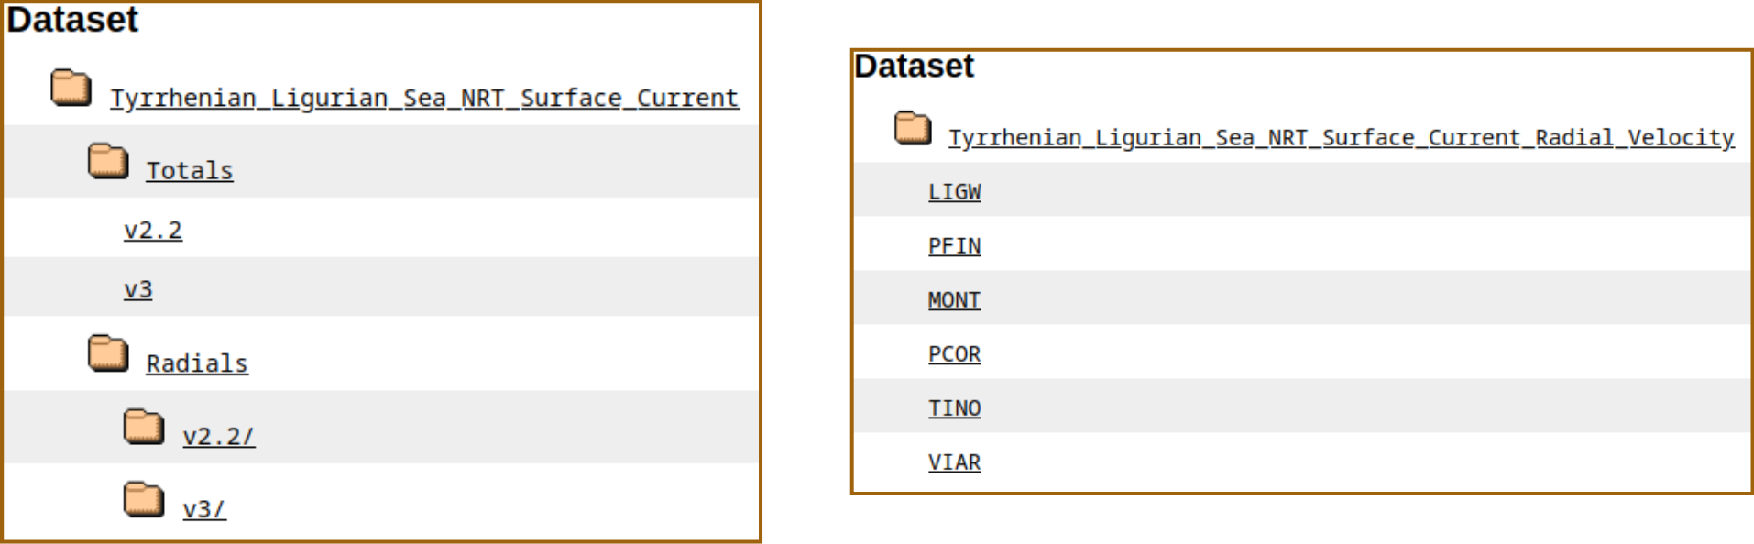
\includegraphics[width=\textwidth]{images/hfr_catalog.pdf}
\captionsetup{font=small, hypcap=false}
\captionof{figure}{Dataset HFR. Distinzione tra dati totali e radiali all'interno del catalogo. I dati radiali avranno un'ulteriore divisione in sottocartelle, una per ogni radar presente nel sistema (figura a destra), mentre i dati totali visualizzeranno direttamente le informazioni sui dati.\footcite[Fonte: ][\url{https://thredds.hfrnode.eu:8443/thredds/NRTcurrent/HFR-TirLig/HFR-TirLig_catalog.html}]{thredds-hfr-trilig}.}
\label{fig:hfr_catalog}
\end{minipage}
\vspace{0.25cm}
\end{figure}

Tra le tante variabili osservate\footcite[40-50]{HFR_QC_JERICO}, le uniche rilevanti risultano essere la velocità dell'acqua del mare in superficie verso est --  \textit{surface eastward sea water velocity} -- (\textbf{EWCT}) e la velocità del mare in superficie verso nord -- \textit{surface northward sea water velocity} -- (\textbf{NSCT}), misurate entrambe in metri al secondo ($m*s^{-1}$). Vengono impiegate, come da standard meteorologico, nel calcolo del vento\footcite[\url{https://confluence.ecmwf.int/pages/viewpage.action?pageId=111155337}]{website-ecmwf-confluence}.



\end{document}